% Bài báo #1 - bản thảo tiếng Việt (P1.10, Khung A, 2026-10-08). Cùng nội
% dung, số liệu, hình và trích dẫn với main_en.tex.
% Biên dịch: tectonic main_vi.tex   (XeTeX + BibTeX, xem README.md)
% Mọi số liệu: pipeline không cân bằng cạnh tuần hoàn (quyết định C5).
% Bản trước: archive/main_vi_2026-09-30.tex.
\documentclass[a4paper,11pt]{article}

\usepackage{fontspec}
\setmainfont{texgyretermes}[Extension=.otf,UprightFont=*-regular,BoldFont=*-bold,ItalicFont=*-italic,BoldItalicFont=*-bolditalic]
\usepackage[english,vietnamese]{babel}
\setlength{\emergencystretch}{2em}
\usepackage{amsmath,amssymb}
\usepackage{icomma} % dấu phẩy thập phân trong công thức: 0,874
\usepackage{graphicx}
\usepackage{booktabs}
\usepackage{multirow}
\usepackage[margin=2.4cm]{geometry}
\usepackage[numbers,sort&compress]{natbib}
\usepackage{caption}
\captionsetup{font=small,labelfont=bf}
\usepackage{tikz}
\usetikzlibrary{arrows.meta,positioning,fit}
\usepackage[colorlinks=true,linkcolor=blue!50!black,citecolor=blue!50!black,urlcolor=blue!50!black]{hyperref}

\newcommand{\nuot}{\nu_{12}}
\newcommand{\nuto}{\nu_{21}}
\newcommand{\RR}{R^2}
% babel đặt lại caption khi vào document -> ghi đè qua \captionsvietnamese.
\addto\captionsvietnamese{%
  \renewcommand{\refname}{Tài liệu tham khảo}%
  \renewcommand{\figurename}{Hình}%
  \renewcommand{\tablename}{Bảng}%
  \renewcommand{\abstractname}{Tóm tắt}%
  \renewcommand{\appendixname}{Phụ lục}}

\title{Tối ưu chính cái được kiểm chứng: tinh chỉnh không gian ẩn nhận biết
nhị phân hóa cho thiết kế ngược vật liệu meta auxetic bằng mô hình sinh}
\author{Trịnh Bình Minh\thanks{[Đơn vị công tác và thông tin tác giả liên hệ - sẽ bổ sung.]}}
\date{Bản thảo, 08/10/2026}

\begin{document}
\maketitle

\begin{abstract}
Thiết kế ô cơ sở vật liệu meta bằng phương pháp gradient, dù là tối ưu
tô-pô hay tìm kiếm trong không gian ẩn của một mô hình sinh, đều được đánh
giá bằng phân tích phần tử hữu hạn (FE) trên thiết kế đã nhị phân hóa, nhưng
thường lại tối ưu một trường mật độ liên tục. Chúng tôi chỉ ra rằng sự lệch
này bị khai thác một cách có hệ thống. Tinh chỉnh mã ẩn của một bộ mã hóa
tự động biến phân có điều kiện (cVAE) theo độ nhạy đồng nhất hóa chính xác
đưa hàm mục tiêu về $\sim\!10^{-10}$, trong khi sai số kiểm chứng vẫn lớn hơn
sáu bậc; tối ưu tô-pô theo mật độ với phép chiếu Heaviside tăng dần tới
$\beta=64$ cũng có cùng khoảng lệch. Đưa các phép biến đổi của khâu kiểm
chứng vào hàm mục tiêu nâng $\RR$ kiểm chứng FE của hệ số Poisson $\nuot$
của ô auxetic hai chiều từ 0,874 lên 0,999 với mẫu đơn (0,831 lên 0,989
trên một tập mục tiêu thứ hai, không giao nhau) và giảm sai số sau chọn
tốt nhất trong 30 mẫu từ 59--68\% trên ba tập rời nhau. So với tối ưu tô-pô
chạy từ đầu với bốn tô-pô khởi tạo, pipeline sinh đạt cùng độ chính xác với
số lần giải FE ít hơn khoảng tám lần và, với mục tiêu dị hướng vừa phải, sai
số cặp $(\nuot,\nuto)$ thấp hơn 35--41\%. Pipeline thất bại với mục tiêu dị
hướng mạnh vốn thưa trong dữ liệu huấn luyện, và tối ưu tô-pô vẫn vượt trội
về khả năng chế tạo và với mục tiêu ngoài dải huấn luyện. Cả hai phương pháp
đôi khi trả về ô suy biến mà một bộ kiểm chứng không có cơ chế bảo vệ vẫn
chấp nhận, nên kiểm tra suy biến phải là một phần của kiểm chứng.
\end{abstract}

\noindent\textbf{Từ khóa:} Vật liệu meta auxetic; Đồng nhất hóa ngược; Tối
ưu tô-pô; Mô hình sinh sâu; Phép chiếu Heaviside; Kiểm chứng

% ---------------------------------------------------------------------------
\section{Mở đầu}

Vật liệu meta auxetic co ngang khi bị nén dọc trục. Hệ số Poisson âm của
chúng bắt nguồn từ vi kiến trúc chứ không từ thành phần hóa học của vật liệu
nền \citep{lakes1987foam,evans2000auxetic,bertoldi2017flexible}. Đồng nhất
hóa ngược bằng tối ưu tô-pô là con đường kinh điển đi từ một ten-xơ hiệu dụng
cho trước tới một ô cơ sở
\citep{sigmund1994materials,larsen1997design,bendsoe2003topology}, nhưng mỗi
mục tiêu mới đòi hỏi một bài toán tối ưu lặp với hàng trăm lần giải FE. Thiết
kế ngược dựa trên dữ liệu khấu hao chi phí này: bộ mã hóa tự động biến phân,
mạng đối nghịch sinh và mô hình khuếch tán huấn luyện trên thư viện mô phỏng
trả về kiến trúc ứng viên gần như tức thì
\citep{wang2020deep,mao2020gan,kumar2020spinodoid,bastek2022inverting,kollmann2020deep,zheng2021controllable,pahlavani2024deep,bastek2023diffusion}.
Mạng nơ-ron cũng đi trực tiếp vào tối ưu tô-pô, dưới dạng tham số hóa lại
trường mật độ \citep{hoyer2019neural,chandrasekhar2021tounn}; một tổng quan
phản biện về các cách tiếp cận này cho thấy nhiều cải thiện được báo cáo biến
mất khi so với tối ưu kinh điển được tinh chỉnh tốt \citep{woldseth2022use}.

Thứ được chế tạo là phiên bản đã nhị phân hóa và lấy mẫu lại của một trường
mật độ, nên độ chính xác phải được đánh giá bằng phân tích FE trên chính
thiết kế đó, không phải bằng mô hình thay thế học được hay bằng trường liên
tục. Mô hình thay thế của ánh xạ thuận được biết là có thể bị bộ tối ưu và
mô hình sinh khai thác \citep{trabucco2021coms}, và một mẫu đơn hiếm khi đạt
dung sai chặt, nên các pipeline sinh nhiều ứng viên rồi chọn bằng FE
\citep{pahlavani2024deep}. Bước tự nhiên tiếp theo là tinh chỉnh thiết kế
được chọn bằng gradient của một bộ giải chính xác. Chúng tôi chỉ ra rằng bước
này thất bại theo một cách đáng học hỏi: bộ tối ưu khai thác các mật độ trung
gian không sống sót qua nhị phân hóa, đúng như cách nó khai thác một mô hình
thay thế thiếu chính xác. Điều tương tự xảy ra với tối ưu tô-pô dùng phép
chiếu Heaviside tăng dần.

Bài báo có các đóng góp sau.
\begin{enumerate}
\item \textbf{Khoảng lệch giữa hàm mục tiêu và kiểm chứng.} Chúng tôi đưa ra
bằng chứng trực tiếp rằng tìm kiếm bằng gradient trên trường mật độ, trong
không gian ẩn của mô hình sinh cũng như trên mật độ phần tử của tối ưu tô-pô,
đạt hàm mục tiêu gần 0 trên những trường có sai số kiểm chứng lớn hơn nhiều
bậc.
\item \textbf{Tinh chỉnh không gian ẩn nhận biết nhị phân hóa.} Đưa các phiên
bản khả vi của các phép biến đổi kiểm chứng (phép chiếu Heaviside tăng dần
\citep{guest2004achieving,wang2011projection} và phép lấy mẫu lại chính xác)
vào hàm mục tiêu, đồng thời chọn theo sai số kiểm chứng, đóng phần lớn khoảng
lệch. Cải thiện này được tái lập trên hai tập mục tiêu rời nhau khác.
\item \textbf{So sánh ngang hàng với tối ưu tô-pô chạy từ đầu.} Trên ba tập
100 mục tiêu, cả hai phương pháp được kiểm chứng qua cùng một chuỗi và so
sánh bằng khoảng tin cậy ghép cặp, phân tầng theo độ dị hướng của mục tiêu,
gồm cả một phép xác nhận với tiêu chí đặt trước trên tập mới và một phương án
lai với tiêu chí đặt trước đã thất bại.
\item \textbf{Phạm vi trung thực.} Chúng tôi báo cáo những chỗ pipeline sinh
thua: mục tiêu dị hướng mạnh, khả năng chế tạo, và mục tiêu có dấu hệ số
Poisson chưa từng thấy, nơi nó thắng truy xuất từ thư viện huấn luyện nhưng
không thắng tối ưu tô-pô. Các thí nghiệm loại bỏ có kiểm soát với đầu mạng
Kolmogorov--Arnold (KAN) và bộ giải mã wavelet ẩn (WIRE) cho kết quả âm.
\end{enumerate}

Mọi độ chính xác được báo cáo đều kiểm chứng bằng FE trên thiết kế đã nhị
phân hóa, mọi so sánh kèm khoảng tin cậy bootstrap ghép cặp, và tiêu chí
thành công được ghi lại trước mỗi thí nghiệm (Mục~\ref{sec:stats}).

% ---------------------------------------------------------------------------
\section{Phương pháp}

\subsection{Sinh dữ liệu}
Ô cơ sở được sinh bằng tối ưu tô-pô SIMP
\citep{bendsoe1989optimal,sigmund2001code,andreassen2011efficient} với bộ
lọc mật độ \citep{bourdin2001filters}, điều kiện biên tuần hoàn và đồng nhất
hóa dựa trên năng lượng
\citep{guedes1990preprocessing,andreassen2014homogenization,xia2015design}.
Các hàm mục tiêu auxetic được cực tiểu hóa từ bốn tô-pô khởi tạo (đồng hồ
cát, lục giác, nơ lõm vào, lỗ tròn), dùng cập nhật tiêu chuẩn tối ưu hoặc
phương pháp tiệm cận di động \citep{svanberg1987mma} tùy theo khởi tạo. Các
tham số quá trình (tỉ lệ thể tích, hệ số phạt, bán kính lọc, giới hạn bước,
kích thước lỗ, góc xoay mạng) được sàng lọc bằng lấy mẫu siêu khối Latin
\citep{mckay1979lhs} rồi tinh chỉnh trong một thiết kế thí nghiệm nhiều đợt
thích nghi dùng dãy Sobol' \citep{sobol1967distribution} và siêu khối Latin
tối ưu. Mẫu hội tụ dao động, tô-pô suy biến hoặc nhãn ngoài dải vật lý bị
loại. Trường mật độ $50\times50$ được lọc hộp lên ảnh $64\times64$ và gán
nhãn $(\nuot,\nuto)$ đồng nhất hóa. Tập dữ liệu production gồm 13\,624 ô,
chia ngẫu nhiên 70/15/15, phân tầng theo tô-pô khởi tạo và theo năm khoảng
cố định của $\nuot$ để mỗi tập con phủ đủ các khởi tạo và toàn dải $\nuot$
(2\,044 ô kiểm tra). Chỉ sau khi chia, ảnh huấn luyện mới được tăng cường sáu
lần bằng phép quay và phản xạ, hoán đổi $\nuot\leftrightarrow\nuto$ khi quay
$90^{\circ}$, cho 57\,216 mẫu huấn luyện; vì vậy không bản tăng cường nào của
một ô huấn luyện có thể nằm trong tập kiểm định hay kiểm tra. Sinh tập dữ
liệu cần ước tính $2,7$--$3,0\times10^{6}$ lần giải FE (65--72 giờ CPU).

\subsection{Đồng nhất hóa và độ nhạy chính xác}
Trường mật độ $\rho\in[0,1]^{50\times50}$ được rời rạc hóa bằng phần tử tứ
giác song tuyến và nội suy SIMP cải tiến
$E(\rho)=E_{\min}+\rho^{p}(E_0-E_{\min})$ với $E_{\min}=10^{-9}E_0$, $p=3$ và
hệ số Poisson vật liệu nền $\nu_0=0,3$. Độ cứng đồng nhất hóa $\mathbf{Q}$
thu được từ ba trường hợp tải tuần hoàn qua năng lượng tương hỗ phần tử
\citep{xia2015design}. Hệ số Poisson tính từ $\mathbf{S}=\mathbf{Q}^{-1}$ là
$\nuot=-S_{12}/S_{11}$ và $\nuto=-S_{12}/S_{22}$, vẫn đúng với ô bị xoay, dị
hướng hoàn toàn. Vì công thức năng lượng là tự liên hợp, độ nhạy
$\partial\mathbf{Q}/\partial\rho_e$ có được mà không cần giải thêm. Chúng
được lan truyền giải tích qua
$\partial\mathbf{S}=-\mathbf{S}\,(\partial\mathbf{Q})\,\mathbf{S}$ và quy
tắc thương trong một hàm autograd PyTorch \citep{paszke2019pytorch} tự viết,
có gradient khớp sai phân hữu hạn với sai số tương đối dưới $10^{-4}$. Bộ
giải khớp một bản cài đặt scikit-fem độc lập \citep{gustafsson2020skfem} tới
$10^{-9}$ trên 24 thiết kế. Một lần giải kèm độ nhạy mất 0,086\,s.

\subsection{cVAE}
cVAE \citep{kingma2014vae,sohn2015cvae} được điều kiện hóa theo
$c=(\nuot,\nuto)$ và có không gian ẩn 32 chiều. Bộ mã hóa gồm bốn khối
tích chập--chuẩn hóa batch--ReLU--pooling (32 tới 256 kênh) giữ bản đồ không
gian $4\times4$, tiếp theo là các lớp tuyến tính cho trung bình và
log-phương sai. Bộ giải mã đối xứng với bộ mã hóa, dùng tích chập chuyển vị
và đầu ra sigmoid. Giai đoạn 1 huấn luyện với tái tạo cross-entropy nhị
phân, số hạng KL khởi động tuyến tính \citep{bowman2016generating} và số hạng
nhất quán tính chất từ một mô hình thay thế tích chập đóng băng (trọng số
$\gamma=20$; $\RR$ kiểm tra của mô hình thay thế là 0,974 cho $\nuot$ và
0,964 cho $\nuto$). Giai đoạn 2 tiếp tục từ giai đoạn 1 và thêm sai số bình
phương giữa $c$ và hệ số Poisson đồng nhất hóa FE của các mẫu \emph{tiên
nghiệm} $z\sim\mathcal N(0,I)$ đã giải mã (trọng số 20; 8 mẫu mỗi hai
epoch). Đây chính là chế độ dùng khi suy luận, và huấn luyện với hàm mất mát
này từ đầu thì thất bại. Tối ưu dùng Adam \citep{kingma2015adam}. Checkpoint
được chọn theo $\RR$ kiểm chứng FE trên các điều kiện kiểm định chứ không
theo mất mát kiểm định, vốn không tin cậy do khởi động KL.

\subsection{Kiểm chứng, suy biến và khả năng chế tạo}
\label{sec:verify}
Một ảnh giải mã được kiểm chứng qua (1) ngưỡng 0,5; (2) lấy mẫu lại láng
giềng gần nhất về $50\times50$ với đúng bản đồ chỉ số của thư viện ảnh dùng
khi dựng tập dữ liệu; và (3) đồng nhất hóa FE. Điều kiện biên tuần hoàn trên
lưới phần tử khiến mọi ô điểm ảnh đều lát kín mặt phẳng bằng phép tịnh tiến,
nên không cần khớp các cạnh đối diện. Một phiên bản trước của pipeline lấy
trung bình các hàng và cột biên đối diện trước khi lấy ngưỡng; chúng tôi bỏ
bước này vì nó làm thay đổi điểm ảnh biên mà không cần cho việc lát
(Phụ lục~\ref{app:fp}). Một thiết kế đã kiểm chứng được gọi là \emph{suy
biến} nếu $\min(E_1,E_2)<10^{-3}E_0$, tức không có đường truyền lực theo ít
nhất một phương; ô như vậy được tính là thất bại trong mọi phân tích nhưng
vẫn giữ trong mọi giá trị trung bình.

Một thiết kế được coi là chế tạo được nếu pha rắn là một thành phần liên
thông duy nhất (liên thông 8) và không thành phần nào biến mất sau phép co
hình thái một điểm ảnh, tức không có thanh nào mảnh hơn hai điểm ảnh. Với ô
cạnh $L$, đây là kích thước nét tối thiểu $0,04L$, ví dụ 0,4\,mm cho ô
10\,mm, tương đương đường kính đầu phun của máy in đùn sợi để bàn. Vì liên
thông 8 chấp nhận tiếp xúc chỉ tại góc (bản lề một nút), chúng tôi kiểm tra
mức độ phổ biến của chúng trong dữ liệu huấn luyện: 17\% ảnh có ít nhất một
bản lề như vậy, nhưng tỉ lệ này là 28\% ở các ô có $|\nuot|$ nhỏ và 3\% ở các
ô có $|\nuot|$ lớn, nên các hệ số Poisson cực trị trong dữ liệu không đến từ
bản lề.

Trong các ứng viên cho một mục tiêu, pipeline chọn hoặc theo sai số cặp kiểm
chứng $|\Delta\nuot|+|\Delta\nuto|$ (Mục~\ref{sec:acc}--\ref{sec:simp}) hoặc
theo điểm tổng hợp
$0,6\,s_{\mathrm{acc}}+0,3\,s_{\mathrm{man}}+0,1\,s_{\mathrm{aes}}$
(Mục~\ref{sec:multi}). Điểm chính xác $s_{\mathrm{acc}}$ là $|\Delta\nuot|$
chuẩn hóa min--max trong tập ứng viên, đảo dấu; $s_{\mathrm{man}}$ là trung
bình của hai chỉ báo liên thông và kích thước nét; điểm thẩm mỹ
$s_{\mathrm{aes}}$ lấy trung bình độ đối xứng gương theo hai trục và nghịch
đảo tỉ số chu vi trên diện tích chuẩn hóa có quấn tuần hoàn. Các trọng số
mã hóa thứ tự ưu tiên; chúng là lựa chọn thiết kế chứ không phải đại lượng
học được.

\subsection{Tinh chỉnh không gian ẩn}
Cho $\boldsymbol\nu^{*}$ và mã ẩn khởi đầu $z_0$ (mẫu đơn hoặc ứng viên thắng
trong best-of-$N$), tinh chỉnh nhận biết nhị phân hóa cực tiểu hóa
\begin{equation}
\mathcal L_\beta(z)=\tfrac12\bigl\lVert
\boldsymbol\nu\bigl(\mathcal R\circ H_\beta\circ D(z,c)\bigr)
-\boldsymbol\nu^{*}\bigr\rVert_2^2 ,
\end{equation}
trong đó $D$ là bộ giải mã đóng băng, $\mathcal R$ là phép lấy mẫu lại láng
giềng gần nhất cài đặt dưới dạng phép gather khả vi với cùng bản đồ chỉ số
của bộ kiểm chứng, và
\begin{equation}
H_\beta(\rho)=\frac{\tanh(\beta\eta)+\tanh\bigl(\beta(\rho-\eta)\bigr)}
{\tanh(\beta\eta)+\tanh\bigl(\beta(1-\eta)\bigr)},\qquad \eta=0,5,
\end{equation}
là phép chiếu Heaviside làm trơn \citep{wang2011projection}. Ba mươi hai bước
L-BFGS \citep{liu1989lbfgs} (bước 0,5, tìm kiếm đường strong-Wolfe) được chia
đều cho $\beta\in\{1,4,16,64\}$, và L-BFGS được khởi động lại ở mỗi mức vì
thông tin độ cong từ phép chiếu mềm hơn không dùng lại được. Baseline liên
tục áp hàm mất mát lên $D(z,c)$ với lấy mẫu lại song tuyến trong 30 bước.
Tinh chỉnh có kiểm soát (guarded) chỉ giữ thiết kế đã tinh chỉnh nếu sai số
cặp kiểm chứng của nó nhỏ hơn của điểm xuất phát.

\subsection{Baseline tối ưu tô-pô và phương án lai}
\label{sec:to}
Với mỗi mục tiêu, chúng tôi cực tiểu hóa
$\tfrac12\lVert\boldsymbol\nu(\hat{\mathbf x})-\boldsymbol\nu^{*}\rVert_2^2$
theo mật độ phần tử $\mathbf x$, với $\hat{\mathbf x}=H_\beta(\tilde{\mathbf x})$
và $\tilde{\mathbf x}$ là trường đã lọc mật độ (bán kính 1,5 phần tử), chịu
ràng buộc $\overline{\hat{\mathbf x}}\le0,55$ và
$Q_{11},Q_{22}\ge0,1\cdot0,55\,E_0$, dùng phương pháp tiệm cận di động
\citep{svanberg1987mma} với hệ số phạt $p=3$. Độ nhạy lấy từ cùng các biểu
thức giải tích dùng cho tinh chỉnh. Quá trình tăng dần chạy
$\beta\in\{1,2,4,8,16,32,64\}$ với tối đa 43 lần đánh giá mỗi mức và khởi
động lại bộ tối ưu ở mỗi mức. Bốn tô-pô khởi tạo của dữ liệu huấn luyện làm
điểm xuất phát, được co giãn về giới hạn thể tích. $\hat{\mathbf x}$ cuối
được lấy ngưỡng 0,5 và kiểm chứng bằng một lần giải FE độc lập, y như một
thiết kế sinh ra, và khởi tạo tốt nhất trong bốn được chọn theo sai số cặp
kiểm chứng. Tham số quá trình là trung vị của dữ liệu huấn luyện. Một biến
thể cùng ngân sách cho phép tối đa 105 lần đánh giá mỗi khởi tạo. Phương án
lai dùng thiết kế nhị phân được sinh làm điểm xuất phát và
$\beta\in\{8,16,32,64\}$ với tối đa 15 lần đánh giá mỗi mức.

\subsection{Truy xuất và giao thức ngoài phân phối}
Truy xuất trả về các ô huấn luyện có khoảng cách Euclid nhỏ nhất tới mục tiêu
trong không gian nhãn $(\nuot,\nuto)$; mỗi ảnh truy xuất được kiểm chứng qua
cùng chuỗi như ảnh sinh, hoặc chỉ ô gần nhất, hoặc ô tốt nhất theo sai số
kiểm chứng trong 30 ô gần nhất. Với mục tiêu $\nuot^{*}>0$ (thí nghiệm đổi
dấu), chúng tôi dùng 28 mục tiêu trong ba nhóm: đối xứng
$\nuot^{*}=\nuto^{*}\in\{0,05;\dots;0,60\}$ (12 mục tiêu) và
$\nuot^{*}\in\{0,05;\dots;0,80\}$ với $\nuto^{*}=0,1$ hoặc $0,3$ (mỗi nhóm 8
mục tiêu). Phép quét biên độ dùng sáu mục tiêu dị hướng với
$\nuto^{*}=-0,05$ và mười lần lặp độc lập của best-of-30 cho mỗi mục tiêu.
Tính chấp nhận được kiểm theo điều kiện $\nuot\nuto<1$
\citep{lempriere1968poisson}.

\subsection{Thống kê và tiêu chí đặt trước}
\label{sec:stats}
Các tập mục tiêu trong phân phối A, B và C mỗi tập gồm 100 điều kiện kiểm
tra, rút với seed 123, 456 và 789 (A và B trùng nhau 4 điều kiện). Mức giảm
MAE tương đối và CI 95\% được tính bằng bootstrap phân vị ghép cặp trên các
điều kiện với 10\,000 lần lấy mẫu lại \citep{efron1993bootstrap}. Một cải
thiện chỉ được khẳng định nếu CI không chứa 0. Tiêu chí thành công được ghi
vào kế hoạch dự án trước khi chạy mỗi thí nghiệm (đặt trước; kế hoạch được
quản lý phiên bản trong kho mã). Các tiêu chí gồm: giảm MAE ít nhất 20\% cho
mẫu đơn; không tăng MAE có ý nghĩa sau best-of-30; sai số tương đối trung vị
không quá 8\% tại $\nuot^{*}=-2,0$; tương quan Spearman trung bình ít nhất
0,7 cho điểm tổng hợp; với KAN, CI không chứa 0 ở cả hai seed; với WIRE, tỉ
lệ trúng ít nhất 30\% và $\RR$ FE $>0$; với phương án lai, sai số cặp không
kém hơn quá 10\% so với tối ưu tô-pô hội tụ, ít nhất 70\% chế tạo được, tối
đa 299 lần giải FE mỗi mục tiêu và tối đa 1\% thiết kế suy biến; và với phép
so sánh phân tầng trên tập C, CI loại trừ 0 theo hướng có lợi cho pipeline
sinh cho cả sai số cặp và sai số $\nuot$ khi tỉ số dị hướng $r<10$. Tập A và
B đã được phân tích trước khi nghĩ tới việc phân tầng, nên kết quả phân tầng
trên hai tập này là hậu kiểm. Phương pháp tinh chỉnh được xây dựng sau khi
tinh chỉnh liên tục thất bại trên tập A; tập B và C đóng vai trò xác nhận.
L-BFGS trên GPU không tất định từng bit, và các lần chạy lặp lệch nhau
khoảng 0,006 về $\RR$.

% ---------------------------------------------------------------------------
\section{Kết quả}

\subsection{Pipeline và giao thức đánh giá}

Hình~\ref{fig:framework} trình bày pipeline. cVAE ánh xạ cặp mục tiêu
$(\nuot^{*},\nuto^{*})$ và các vector ẩn $z\sim\mathcal N(0,I)$ thành ảnh
mật độ $64\times64$. Mỗi ảnh được nhị phân hóa, lấy mẫu lại về lưới FE và
đồng nhất hóa. Ứng viên tốt nhất được tinh chỉnh trong không gian ẩn, và
thiết kế đã tinh chỉnh chỉ được giữ nếu sai số kiểm chứng của nó thấp hơn
(tinh chỉnh ``có kiểm soát''). Mọi số liệu dưới đây đều kiểm chứng bằng FE
trên thiết kế đã nhị phân hóa.

\begin{figure}[t]
\centering
\begin{tikzpicture}[
  node distance=3mm and 4mm,
  box/.style={draw, rounded corners=2pt, align=center, font=\small,
              minimum height=10mm, inner sep=3pt, fill=#1},
  box/.default=white,
  arr/.style={-{Stealth[length=2mm]}, thick}]
\node[box=gray!10] (t) {mục tiêu\\$(\nu_{12}^{*},\nu_{21}^{*})$\\$z_{1..N}\!\sim\!\mathcal N(0,I)$};
\node[box=orange!15, right=of t] (g) {bộ giải mã\\cVAE (tinh\\chỉnh vật lý)};
\node[box=blue!8, right=of g] (v) {ngưỡng 0,5\\lấy mẫu $50^2$};
\node[box=green!12, right=of v] (fe) {đồng nhất\\hóa FE\\kiểm suy biến};
\node[box=yellow!15, right=of fe] (s) {chọn (sai số\\kiểm chứng hoặc\\điểm tổng hợp)};
\node[box=blue!15, right=of s] (r) {tinh chỉnh\\ẩn có\\kiểm soát};
\draw[arr] (t) -- (g);
\draw[arr] (g) -- (v);
\draw[arr] (v) -- (fe);
\draw[arr] (fe) -- (s);
\draw[arr] (s) -- (r);
\draw[arr, dashed] (r.north) -- ++(0,5mm) -| node[pos=0.25, above, font=\scriptsize]{kiểm chứng lại thiết kế đã tinh chỉnh} (fe.north);
\end{tikzpicture}
\caption{Pipeline thiết kế ngược. Mọi ứng viên được kiểm chứng bằng đồng nhất
hóa FE sau đúng các bước hậu xử lý mà một thiết kế được chế tạo phải trải
qua. Bước tinh chỉnh được mô tả ở Hình~\ref{fig:pipeline}.}
\label{fig:framework}
\end{figure}

\subsection{Độ chính xác đã kiểm chứng đòi hỏi tối ưu chính thiết kế được kiểm chứng}
\label{sec:acc}

\paragraph{Tinh chỉnh liên tục khai thác vật liệu xám.}
Tinh chỉnh đầu ra liên tục của bộ giải mã (30 bước L-BFGS, gradient qua bộ
giải mã và độ nhạy đồng nhất hóa chính xác) giúp mẫu đơn của mô hình
production. Trên tập A, $\RR(\nuot)$ tăng từ 0,874 lên 0,976 và sai số tuyệt
đối trung bình (MAE) của $\nuot$ giảm 57,7\% (CI 95\% 49,4--64,6\%;
Bảng~\ref{tab:main}, Hình~\ref{fig:parity}b). Tuy nhiên, cùng phép tinh chỉnh
đó lại \emph{làm xấu đi} ứng viên thắng của best-of-30: MAE($\nuot$) tăng từ
0,0142 lên 0,0247, tức thay đổi $-73,8\%$ (CI $-119$ tới $-39\%$), và $\RR$
giảm từ 0,988 xuống 0,962. Quỹ đạo hàm mục tiêu giải thích lý do
(Hình~\ref{fig:gap}). Cuối tinh chỉnh liên tục, trung vị hàm mục tiêu là
$2,5\times10^{-10}$, nhưng trung vị sai số bình phương kiểm chứng của thiết
kế đã nhị phân hóa là $4,4\times10^{-4}$. Bộ tối ưu khớp mục tiêu trên một
trường có các mật độ trung gian không sống sót qua phép lấy ngưỡng
(Hình~\ref{fig:refex}). Đây là kiểu thất bại của việc khai thác mô hình thay
thế, nhưng xuất hiện bên trong một mô hình vật lý chính xác.

\paragraph{Tinh chỉnh nhận biết nhị phân hóa.}
Đưa các phiên bản khả vi của các phép biến đổi kiểm chứng vào hàm mục tiêu
(Hình~\ref{fig:pipeline}) thu hẹp trung vị tỉ số giữa sai số kiểm chứng và
hàm mục tiêu từ khoảng $10^{6}$ xuống khoảng $2\times10^{2}$
(Hình~\ref{fig:gap}). Mọi tiêu chí đặt trước trong phân phối đều đạt
(Bảng~\ref{tab:main}).
\begin{itemize}
\item \textbf{Mẫu đơn.} $\RR(\nuot)$ tăng từ 0,874 lên 0,999 và MAE($\nuot$)
giảm 92,7\% (CI 90,2--94,6\%). Sai số tương đối trung bình của $\nuot$ giảm
từ 14,4\% xuống 2,3\%, và $\RR(\nuto)$ tăng từ 0,477 lên 0,875.
\item \textbf{Sau best-of-30.} MAE($\nuot$) giảm 68,3\% (CI 59,3--75,8\%),
$\RR(\nuot)$ tăng từ 0,988 lên 0,998, và MAE($\nuto$) giảm từ 0,030 xuống
0,010 ($\RR(\nuto)$ từ 0,812 lên 0,845). Tinh chỉnh có kiểm soát chấp nhận
94\% kết quả tinh chỉnh và cho cùng độ chính xác.
\end{itemize}
Tinh chỉnh tốn trung bình 77 lần giải FE mỗi mục tiêu, tức khoảng 7\,s CPU
trên lưới $50\times50$. Riêng cơ chế kiểm soát không cứu được tinh chỉnh liên
tục sau best-of-30 (MAE giảm 10,5\%, CI $-3,0$ tới 22,4\%).

\paragraph{Tái lập trên các tập mục tiêu mới.}
Vì phương pháp được xây dựng sau khi tinh chỉnh liên tục thất bại trên tập A,
chúng tôi lặp lại nó trên tập B và C, rút với seed khác. Với mẫu đơn trên tập
B, $\RR(\nuot)$ tăng từ 0,831 lên 0,989 và MAE($\nuot$) giảm 87,8\% (CI
82,3--92,3\%). Sau best-of-30, MAE($\nuot$) giảm 59,3\% (CI 46,8--70,9\%)
trên tập B và 63,6\% (CI 46,3--75,2\%) trên tập C.

\begin{figure}[t]
\centering
\begin{tikzpicture}[
  node distance=4mm and 5mm,
  box/.style={draw, rounded corners=2pt, align=center, font=\small,
              minimum height=9mm, inner sep=3pt, fill=#1},
  box/.default=white,
  arr/.style={-{Stealth[length=2mm]}, thick},
  grad/.style={-{Stealth[length=2mm]}, thick, dashed, blue!60!black}]
\node[box=gray!10] (z) {mã ẩn $z$\\(khởi đầu ấm)};
\node[box=gray!10, below=of z] (c) {mục tiêu\\$(\nu_{12}^{*},\nu_{21}^{*})$};
\node[box=orange!15, right=8mm of z, yshift=-6.5mm] (dec) {bộ giải mã\\cVAE đóng băng};
\node[box=blue!8, right=of dec] (hv) {Heaviside\\$H_\beta(\rho)$};
\node[box=blue!8, right=of hv] (rs) {láng giềng\\$64^2\!\to\!50^2$};
\node[box=green!12, right=of rs] (fe) {đồng nhất hóa FE\\$\mathbf{Q}\to\nu_{12},\nu_{21}$};
\node[box=gray!10, below=9mm of rs] (loss) {$\mathcal{L}=\tfrac12\lVert\boldsymbol{\nu}-\boldsymbol{\nu}^{*}\rVert^2$};
\draw[arr] (z) -| ([xshift=-3mm]dec.west) -- (dec.west);
\draw[arr] (c) -| ([xshift=-3mm]dec.west);
\draw[arr] (dec) -- (hv);
\draw[arr] (hv) -- (rs);
\draw[arr] (rs) -- (fe);
\draw[arr] (fe.south) |- (loss.east);
\draw[grad] (loss.west) -- ([xshift=-6mm]loss.west -| z.west)
  node[pos=0.45, below, font=\scriptsize]{$\partial\mathcal{L}/\partial z$ chính xác, L-BFGS; $\beta\in\{1,4,16,64\}$}
  |- (z.west);
\node[draw=blue!50, dashed, rounded corners, fit=(hv)(rs), inner sep=2pt,
      label={[font=\scriptsize]above:cùng phép biến đổi với kiểm chứng}] {};
\end{tikzpicture}
\caption{Tinh chỉnh không gian ẩn nhận biết nhị phân hóa. Đầu ra của bộ giải
mã đóng băng đi qua các phiên bản khả vi của các phép biến đổi kiểm chứng
trước khi đồng nhất hóa FE, nên đại lượng được tối ưu chính là đại lượng
được kiểm chứng. Biến thể liên tục bỏ khối nét đứt và dùng lấy mẫu lại song
tuyến. Khâu kiểm chứng thay $H_\beta$ bằng ngưỡng cứng 0,5.}
\label{fig:pipeline}
\end{figure}

\begin{table}[t]
\centering
\caption{Độ chính xác kiểm chứng FE trên tập A (100 mục tiêu kiểm tra, cVAE
production). $\Delta$MAE là mức giảm tương đối của MAE($\nuot$) so với thiết
kế chưa tinh chỉnh cùng chế độ, kèm CI 95\% bootstrap ghép cặp. Giá trị âm
nghĩa là tinh chỉnh làm kết quả tệ hơn. Cặp: trung bình
$|\Delta\nuot|+|\Delta\nuto|$. FE: số lần giải mỗi mục tiêu, kể cả bước
chọn.}
\label{tab:main}
\small
\setlength{\tabcolsep}{3.2pt}
\begin{tabular}{llcccccr}
\toprule
Chế độ & Tinh chỉnh & $\RR(\nuot)$ & MAE($\nuot$) & $\RR(\nuto)$ & Cặp & $\Delta$MAE [CI 95\%] & FE\\
\midrule
\multirow{3}{*}{Mẫu đơn}
 & không                & 0,874 & 0,0517 & 0,477 & 0,127 & -- & 1\\
 & liên tục             & 0,976 & 0,0219 & 0,643 & 0,053 & $+57,7\%$ [49,4; 64,6] & 51\\
 & nhận biết nhị phân   & \textbf{0,999} & \textbf{0,0038} & \textbf{0,875} & \textbf{0,012} & $\mathbf{+92,7\%}$ [90,2; 94,6] & 78\\
\midrule
\multirow{4}{*}{Best-of-30}
 & không                & 0,988 & 0,0142 & 0,812 & 0,044 & -- & 30\\
 & liên tục             & 0,962 & 0,0247 & 0,671 & 0,052 & $-73,8\%$ [$-119$; $-39$] & 79\\
 & nhận biết nhị phân   & \textbf{0,998} & \textbf{0,0045} & 0,845 & 0,014 & $\mathbf{+68,3\%}$ [59,3; 75,8] & 107\\
 & \quad có kiểm soát   & \textbf{0,998} & 0,0046 & \textbf{0,846} & 0,014 & $+67,4\%$ [57,9; 75,3] & 107\\
\bottomrule
\end{tabular}
\end{table}

\begin{figure}[t]
\centering
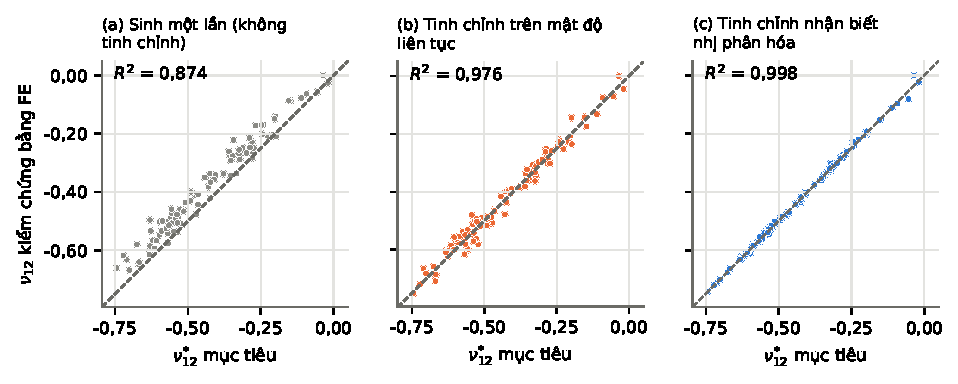
\includegraphics[width=\linewidth]{figures/fig_parity_vi.pdf}
\caption{$\nuot$ kiểm chứng FE theo $\nuot$ mục tiêu trên tập A ($n=100$, mẫu
đơn của cVAE production): (a) chưa tinh chỉnh; (b) sau tinh chỉnh liên tục;
(c) sau tinh chỉnh nhận biết nhị phân hóa. Mọi panel xuất phát từ cùng một mã
ẩn cho mỗi điều kiện. Nét đứt: đường đồng nhất.}
\label{fig:parity}
\end{figure}

\begin{figure}[t]
\centering
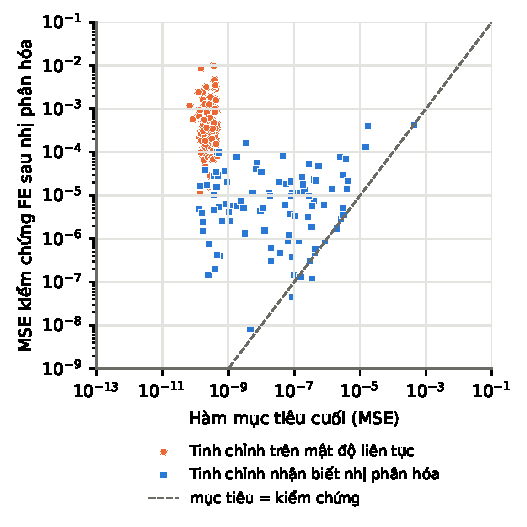
\includegraphics[width=0.55\linewidth]{figures/fig_gap_vi.pdf}
\caption{Khoảng lệch hàm mục tiêu--kiểm chứng. Mỗi điểm là một điều kiện của
tập A. Trục ngang: hàm mục tiêu cuối của tinh chỉnh; trục đứng: sai số bình
phương hệ số Poisson của thiết kế đã nhị phân hóa, đo bằng một lần giải FE
độc lập. Tinh chỉnh liên tục (tròn) đạt hàm mục tiêu gần $10^{-10}$ trong khi
sai số kiểm chứng vẫn ở $10^{-4}$--$10^{-2}$. Tinh chỉnh nhận biết nhị phân
hóa (vuông) kéo các điểm về đường đồng nhất. Giá trị dưới $10^{-14}$ bị kẹp
để hiển thị.}
\label{fig:gap}
\end{figure}

\begin{figure}[t]
\centering
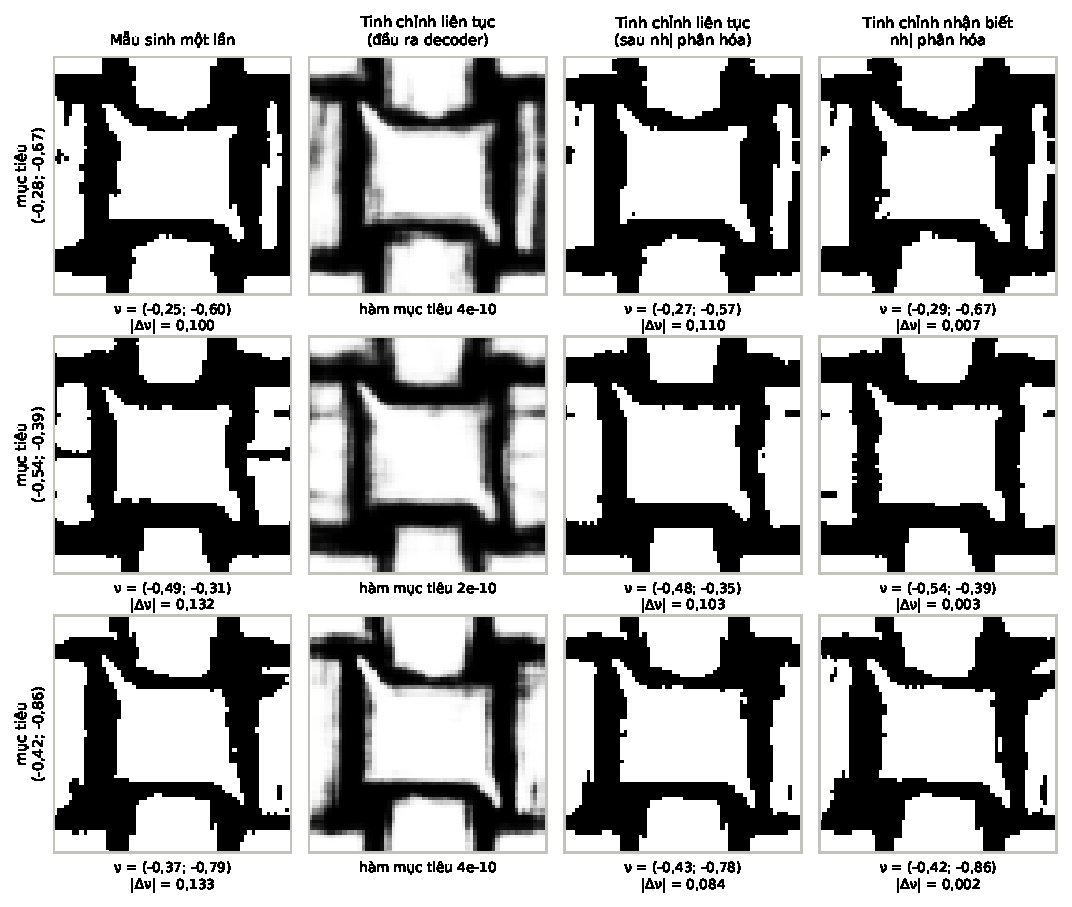
\includegraphics[width=\linewidth]{figures/fig_refine_examples_vi.pdf}
\caption{Cùng một mã ẩn khởi đầu cho ba điều kiện của tập A: mẫu đơn, tinh
chỉnh liên tục (đầu ra bộ giải mã và bản nhị phân hóa của nó), và tinh chỉnh
nhận biết nhị phân hóa (đã nhị phân hóa). Tinh chỉnh liên tục đạt mục tiêu
trên một trường xám mà bản nhị phân hóa của nó có tính chất khác.}
\label{fig:refex}
\end{figure}

\subsection{So sánh với tối ưu tô-pô chạy từ đầu}
\label{sec:simp}

Đối thủ đúng nghĩa của một pipeline sinh không phải là bảng tra mà là tối ưu
tô-pô chạy trực tiếp cho mục tiêu. Chúng tôi giải bài toán đồng nhất hóa
ngược kinh điển cho mọi mục tiêu từ bốn tô-pô khởi tạo (Mục~\ref{sec:to}),
kiểm chứng mỗi kết quả y như một thiết kế sinh ra, và giữ khởi tạo tốt nhất
theo sai số kiểm chứng. Baseline này dùng trung bình 893 lần giải FE mỗi mục
tiêu (trung vị 102--140\,s CPU trên một lõi), so với 107 lần của best-of-30
kèm tinh chỉnh nhận biết nhị phân hóa có kiểm soát.

\paragraph{Tối ưu tô-pô cũng có cùng khoảng lệch.}
Cuối quá trình tăng dần, trung vị sai số trên trường mật độ đã chiếu là
$2\times10^{-7}$, trong khi trung vị sai số kiểm chứng sau lấy ngưỡng là
$3,6\times10^{-2}$ mỗi lần chạy, và với 57\% trong 300 mục tiêu, tô-pô khởi
tạo có sai số trên trường chiếu thấp nhất không phải là tô-pô có sai số kiểm
chứng thấp nhất. Vì vậy chọn theo sai số kiểm chứng là cần thiết cho cả hai
phương pháp.

\paragraph{Độ chính xác, chi phí và kiểu thất bại.}
Bảng~\ref{tab:simp} so sánh hai phương pháp trên tập A, B và C. Trên cả ba
tập, pipeline sinh ngang tối ưu tô-pô hội tụ về $\nuot$ ($\RR=0,995$--$0,998$
so với $0,996$--$0,998$) với số lần giải FE ít hơn khoảng tám lần. Tính trên
mọi mục tiêu, sai số cặp của nó không thấp hơn một cách nhất quán, do một
kiểu thất bại duy nhất. Mọi ô suy biến do cVAE sinh ra (một ở tập A, hai ở
tập B, không có ở tập C) đều thuộc mục tiêu có tỉ số dị hướng
$r=\max(\nuto^{*}/\nuot^{*},\,\nuot^{*}/\nuto^{*})\ge10$, tương ứng tỉ số độ
cứng $E_2/E_1\ge10$ với ô trực hướng. Trong các ô này có một cột điểm ảnh
rỗng, nên ô không chịu lực theo một phương và hệ số Poisson của nó vô nghĩa
(Hình~\ref{fig:designs}). Với các mục tiêu này, cả 30 ứng viên đều bị đứt,
nên không thể sửa bằng bước chọn; chỉ 2,8\% ô huấn luyện có $r>10$. Bỏ ba mục
tiêu suy biến, sai số cặp của pipeline sinh là 0,0075, 0,0091 và 0,0082, so
với 0,0127, 0,0140 và 0,0126 của tối ưu tô-pô, vốn không sinh ô suy biến
nào. $\RR(\nuto)$ thấp của pipeline sinh trên tập A và B (0,846; 0,745) cũng
do chính các mục tiêu này.

\paragraph{Xác nhận phân tầng với tiêu chí đặt trước.}
Sau khi quan sát hiện tượng trên tập A và B, chúng tôi đặt trước một phép
kiểm định phân tầng trên tập C trước khi chạy: với mục tiêu có $r<10$, pipeline
sinh phải có sai số cặp và sai số $\nuot$ thấp hơn tối ưu tô-pô, với CI 95\%
ghép cặp loại trừ 0. Phép kiểm định này được chạy với pipeline cũ còn cân
bằng cạnh tuần hoàn (Phụ lục~\ref{app:fp}). Tiêu chí sai số cặp đạt (thấp hơn
27\%, CI 8--42\%); tiêu chí $\nuot$ không đạt (thấp hơn 19\%, CI $-10$ tới
40\%). Với pipeline cuối, cả hai tiêu chí đều đạt trên cả ba tập
(Bảng~\ref{tab:simp}); vì phiên bản này không được đặt trước, chúng tôi báo
nó như phân tích độ nhạy và chỉ khẳng định ngang bằng về $\nuot$ cùng lợi thế
về sai số cặp cho dị hướng vừa phải, không khẳng định vượt trội về $\nuot$.
Trong năm mục tiêu có $r\ge10$, pipeline sinh tốt hơn ở một (tập C) và kém
hơn nhiều ở bốn.

\begin{table}[t]
\centering
\caption{Pipeline sinh (best-of-30 + tinh chỉnh nhận biết nhị phân hóa có
kiểm soát) so với tối ưu tô-pô chạy từ đầu (tốt nhất trong bốn khởi tạo, hội
tụ) trên ba tập rời nhau, mỗi tập 100 mục tiêu. Cả hai chọn theo sai số cặp
kiểm chứng. Cặp: trung bình $|\Delta\nuot|+|\Delta\nuto|$. FE: số lần giải
mỗi mục tiêu. Suy biến: số ô có $\min E_i<10^{-3}E_0$. Chế tạo: tỉ lệ chế
tạo được. Hai dòng cuối: mức giảm sai số tương đối của pipeline sinh so với
tối ưu tô-pô cho mục tiêu có tỉ số dị hướng $r<10$ (CI 95\% bootstrap ghép
cặp; dương là có lợi cho pipeline sinh).}
\label{tab:simp}
\small
\setlength{\tabcolsep}{3.2pt}
\begin{tabular}{llcccccc}
\toprule
Tập & Phương pháp & $\RR(\nuot)$ & $\RR(\nuto)$ & Cặp & FE & Suy biến & Chế tạo\\
\midrule
\multirow{2}{*}{A} & sinh & 0,998 & 0,846 & 0,0139 & 107 & 1 & 0,32\\
 & tối ưu tô-pô & 0,997 & 0,997 & 0,0128 & 897 & 0 & 0,77\\
\multirow{2}{*}{B} & sinh & 0,995 & 0,745 & 0,0229 & 107 & 2 & 0,35\\
 & tối ưu tô-pô & 0,996 & 0,997 & 0,0139 & 889 & 0 & 0,74\\
\multirow{2}{*}{C} & sinh & 0,998 & 0,998 & 0,0082 & 107 & 0 & 0,32\\
 & tối ưu tô-pô & 0,998 & 0,996 & 0,0126 & 893 & 0 & 0,83\\
\midrule
\multicolumn{8}{l}{$r<10$, sai số cặp: \;A $+41\%$ [26; 54] \;B $+40\%$ [23; 53] \;C $+35\%$ [19; 48]}\\
\multicolumn{8}{l}{$r<10$, sai số $\nuot$: \;A $+39\%$ [19; 54] \;B $+39\%$ [19; 54] \;C $+37\%$ [14; 54]}\\
\bottomrule
\end{tabular}
\end{table}

\begin{figure}[t]
\centering
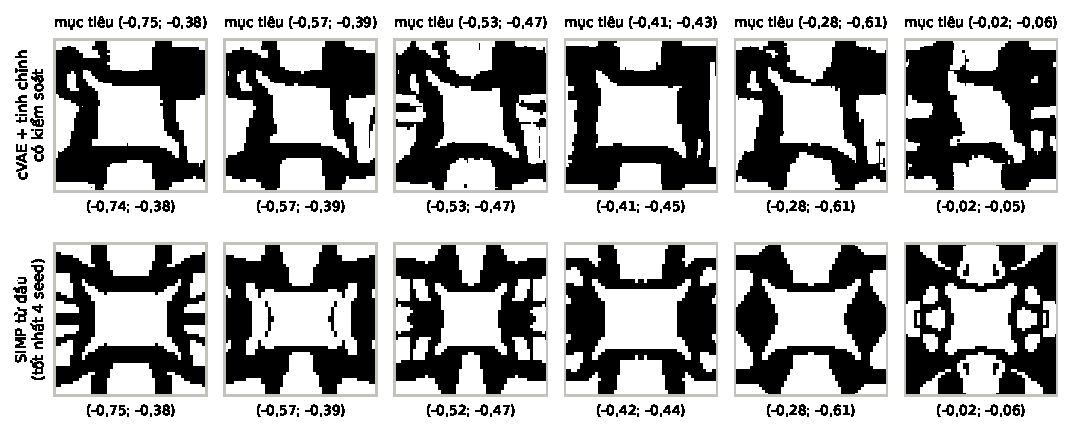
\includegraphics[width=\linewidth]{figures/fig_designs_vi.pdf}
\caption{Thiết kế cuối của pipeline sinh và của tối ưu tô-pô chạy từ đầu cho
cùng các mục tiêu của tập A, kèm $(\nuot,\nuto)$ mục tiêu và kiểm chứng.}
\label{fig:designs}
\end{figure}

\paragraph{Độ nhạy lưới và độ cứng.}
Mọi độ chính xác ở trên đều so với mô hình FE $50\times50$ dùng để sinh dữ
liệu, tinh chỉnh và kiểm chứng. Giải lại 30 hình học kiểm tra với mỗi điểm
ảnh chia thành $4\times4$ phần tử làm $\nuot$ thay đổi trung vị 0,015
(3,8\%) và tối đa 0,042, theo hướng âm hơn ở 27 hình. Do đó chênh lệch
$\nuot$ giữa hai phương pháp ($\sim\!10^{-3}$) nhỏ hơn một bậc so với sai số
rời rạc hóa của mô hình. Trên lưới $200\times200$, thứ hạng của hai phương
pháp trên tập A không đổi ($\RR(\nuot)$ 0,992 so với 0,985).
% TODO(P1.10): số 200^2 và fig_stiffness tính cho biến thể có cân bằng cạnh
% tuần hoàn (p1_6x_final_design_eval.json) - chạy lại khi cắm sạc, xem
% main_en.tex.
Thiết kế auxetic của cả hai phương pháp không phải cơ cấu gần như không có
độ cứng: trung vị mô-đun trong mặt phẳng là $E_1\approx0,07$--$0,08\,E_0$ cho
cả hai (Hình~\ref{fig:stiffness}).

\begin{figure}[t]
\centering
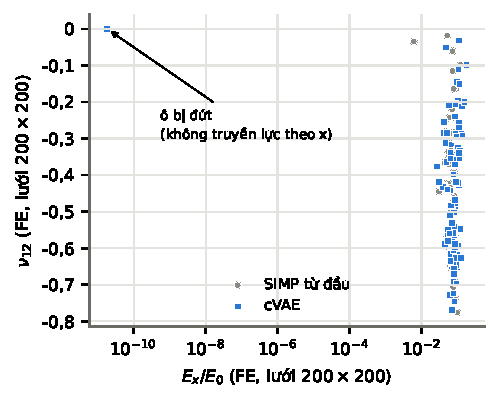
\includegraphics[width=0.6\linewidth]{figures/fig_stiffness_vi.pdf}
\caption{$\nuot$ kiểm chứng theo $E_1/E_0$ của thiết kế cuối trên tập A, cả
hai trên lưới $200\times200$. Giá trị tính cho biến thể pipeline có cân bằng
cạnh tuần hoàn.}
\label{fig:stiffness}
\end{figure}

\paragraph{Phương án lai không thừa hưởng điểm mạnh của cả hai.}
Vì tối ưu tô-pô bền vững hơn và dễ chế tạo hơn còn pipeline sinh rẻ hơn,
chúng tôi đặt trước tiêu chí cho một phương án lai, trong đó thiết kế sinh ra
làm điểm khởi tạo cho tối ưu tô-pô (tăng dần $\beta=8\to64$, tối đa 61 lần
giải FE thêm). Nó đạt tiêu chí chi phí và không suy biến (166 lần giải FE mỗi
mục tiêu; 1\% suy biến) nhưng trượt tiêu chí không-kém-hơn về sai số cặp so
với tối ưu tô-pô hội tụ (cận dưới CI $-96\%$, do đúng một mục tiêu suy biến)
và tiêu chí chế tạo (0,33 so với ngưỡng 0,70). Xuất phát từ một phép chiếu
sắc giữ nguyên tô-pô, kể cả các nét mảnh, của thiết kế sinh ra. Thí nghiệm
này chạy với pipeline cũ có cân bằng cạnh tuần hoàn.

\paragraph{Chi phí.}
Khoản tiết kiệm khoảng 790 lần giải FE mỗi mục tiêu chỉ bù được
$2,7$--$3,0\times10^{6}$ lần giải FE đã dùng để sinh dữ liệu huấn luyện sau
khoảng 3\,500--3\,800 mục tiêu (11\,500--12\,700 nếu so với biến thể cùng
ngân sách của tối ưu tô-pô). Lập luận chi phí vì vậy chỉ đúng khi cần phục
vụ nhiều mục tiêu, không phải cho một thiết kế đơn lẻ.

\subsection{Truy xuất từ thư viện huấn luyện}
\label{sec:retr}
Tra cứu trong thư viện huấn luyện là phương án rẻ nhất. Khi kiểm chứng qua
cùng chuỗi, ô gần nhất đạt $\RR(\nuot)=0,941$ trên tập A, và ô tốt nhất trong
30 ô gần nhất đạt $\RR=0,977$ với sai số cặp 0,035, nhỉnh hơn best-of-30 của
mô hình sinh khi chưa tinh chỉnh (0,988, sai số cặp 0,044). Tinh chỉnh nhận
biết nhị phân hóa đưa pipeline sinh lên $\RR=0,998$ và sai số cặp 0,014.
Tính chất kiểm chứng của một ô huấn luyện cũng khác nhãn của nó: lấy mẫu lại
từ $64^2$ về $50^2$, phạt và nhị phân hóa cộng lại làm $\nuot$ lệch MAE
0,032 trên 150 ô kiểm tra, vì nhãn được tính trên trường SIMP xám. Nhãn cũng
là một đại lượng khác với thứ được kiểm chứng.

\subsection{Khả năng chế tạo và chọn lọc đa mục tiêu}
\label{sec:multi}

Thiết kế chính xác không tự động chế tạo được. Với chọn best-of-30 theo sai
số kiểm chứng và tinh chỉnh có kiểm soát, 32--35\% thiết kế sinh cuối cùng
chế tạo được, so với 74--83\% của tối ưu tô-pô (Bảng~\ref{tab:simp}). Tinh
chỉnh không làm giảm khả năng chế tạo: qua bốn lần chạy (mẫu đơn và best-of-30
trên tập A, best-of-30 trên tập B và C), tỉ lệ chế tạo được tăng 4--7 điểm
phần trăm, với 55 thiết kế trở thành chế tạo được và 33 mất tính chất này
(kiểm định dấu $p=0,025$; hai lần chạy dùng chung tập A).

Để đánh đổi độ chính xác với khả năng chế tạo ngay khi chọn, điểm tổng hợp ở
Mục~\ref{sec:verify} có thể thay cho sai số kiểm chứng. Trên 300 mục tiêu
kiểm tra ($N=30$), chọn theo điểm tổng hợp giữ $\RR(\nuot)=0,988$ (0,997 khi
chỉ chọn theo độ chính xác) trong khi mọi mẫu đầu tiên đều auxetic; 23,8\% số
mẫu sinh ra chế tạo được (Bảng~\ref{tab:multi}). $\RR$ này khác với
Bảng~\ref{tab:main} vì tập mục tiêu và các lần rút mã ẩn khác nhau. Để kiểm
tra phép vô hướng hóa có tôn trọng cấu trúc đa mục tiêu không, chúng tôi tính,
cho 24 mục tiêu với 30 ứng viên mỗi mục tiêu, tương quan Spearman giữa điểm
tổng hợp và tầng sắp xếp không trội trên ba mục tiêu thô
(Hình~\ref{fig:spearman}). Cả 24 tương quan đều dương (0,45--0,86, trung vị
0,746, trung bình 0,718). Tiêu chí đặt trước (trung bình $\ge0,7$) được đặt
cho pipeline cũ và đã trượt với nó (trung bình 0,693); vì vậy chúng tôi coi
điểm tổng hợp phù hợp ở mức vừa phải, không mạnh, với cấu trúc Pareto. Việc
ứng viên được chọn nằm trên mặt Pareto thứ nhất được bảo đảm với trọng số
dương nên không phải là bằng chứng.

Hình~\ref{fig:tiling} cho thấy các ô sinh ra lát kín mà không cần khớp cạnh,
và Hình~\ref{fig:deformation} cho thấy cơ chế biến dạng của một ô auxetic
sinh ra và của một ô sinh ra có $\nuot>0$.

\begin{table}[t]
\centering
\caption{Chọn lọc trên 300 mục tiêu kiểm tra (best-of-30, không tinh chỉnh).
Tỉ lệ trúng: tỉ lệ mục tiêu có mẫu đầu tiên auxetic ($\nuot<0$). Chế tạo
được: tỉ lệ trên toàn bộ mẫu sinh ra.}
\label{tab:multi}
\small
\begin{tabular}{lccc}
\toprule
Cách chọn & $\RR(\nuot)$ & Tỉ lệ trúng, mẫu đầu & Mẫu chế tạo được\\
\midrule
Chỉ theo độ chính xác kiểm chứng & 0,997 & 1,00 & 0,238\\
Điểm tổng hợp                    & 0,988 & 1,00 & 0,238\\
\midrule
\multicolumn{4}{p{0.85\linewidth}}{Điểm tổng hợp so với tầng Pareto (24 mục tiêu $\times$ 30 ứng viên): Spearman trung bình 0,718, trung vị 0,746, khoảng 0,45--0,86; 24/24 dương.}\\
\bottomrule
\end{tabular}
\end{table}

\begin{figure}[t]
\centering
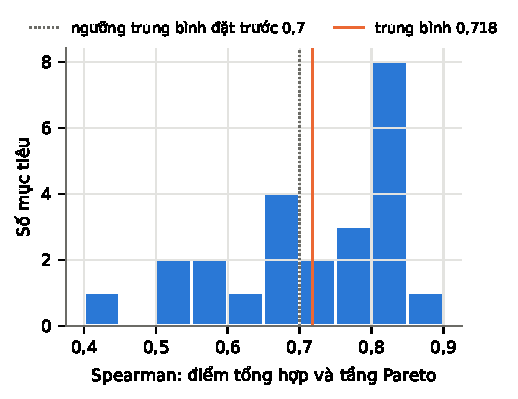
\includegraphics[width=0.5\linewidth]{figures/fig_spearman_vi.pdf}
\caption{Phân bố trên 24 mục tiêu của tương quan Spearman giữa điểm tổng hợp
và tầng Pareto của 30 ứng viên (mục tiêu: $|\Delta\nuot|$ kiểm chứng, điểm
chế tạo, điểm thẩm mỹ). Chấm: ngưỡng đặt trước cho giá trị trung bình.}
\label{fig:spearman}
\end{figure}

\begin{figure}[t]
\centering
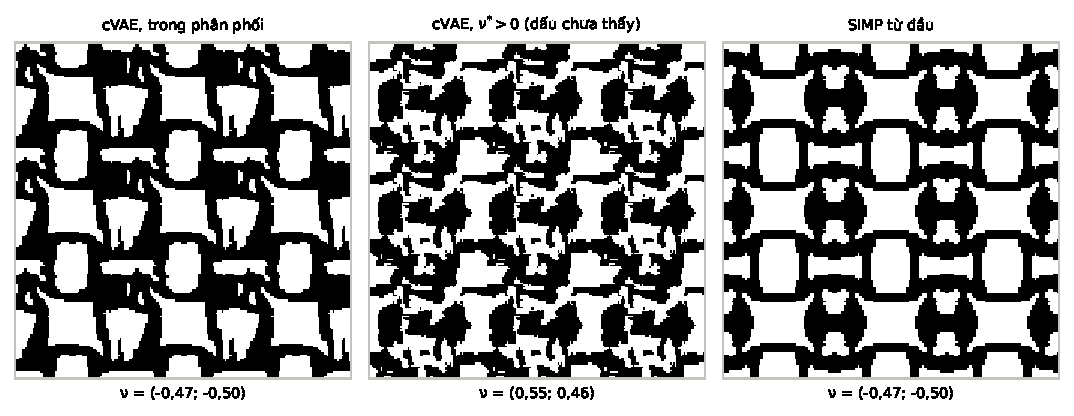
\includegraphics[width=0.85\linewidth]{figures/fig_tiling_vi.pdf}
\caption{Lưới lát $3\times3$ của thiết kế cuối: pipeline sinh trong phân
phối, pipeline sinh với dấu chưa thấy ($\nuot^{*}>0$), và tối ưu tô-pô chạy
từ đầu. Điều kiện biên tuần hoàn trên lưới phần tử khiến mọi ô điểm ảnh lát
kín bằng phép tịnh tiến.}
\label{fig:tiling}
\end{figure}

\begin{figure}[t]
\centering
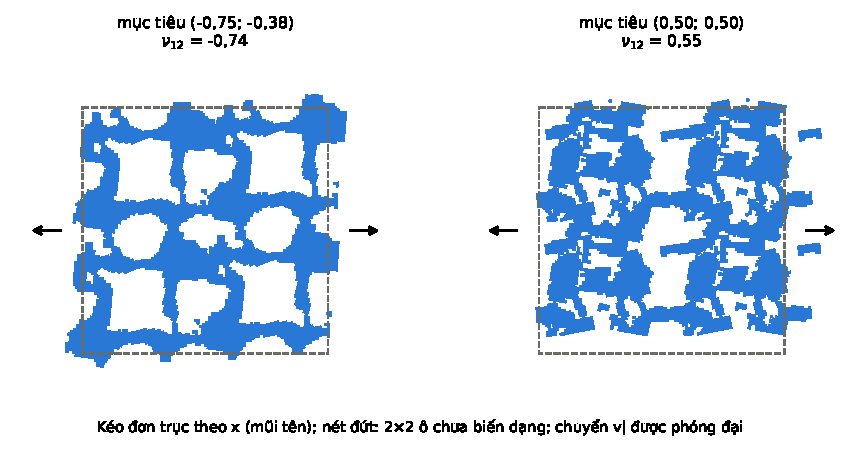
\includegraphics[width=0.85\linewidth]{figures/fig_deformation_vi.pdf}
\caption{Biến dạng dưới kéo đơn trục theo $x$ (FE, $50\times50$, chuyển vị
được phóng đại) của một ô auxetic sinh ra (mục tiêu
$(\nuot^{*},\nuto^{*})=(-0,75;-0,38)$, $\nuot$ kiểm chứng $-0,744$) và của
một ô sinh ra cho $\nuot^{*}=\nuto^{*}=0,5$ (kiểm chứng 0,547). Nét đứt: các
ô $2\times2$ chưa biến dạng.}
\label{fig:deformation}
\end{figure}

\subsection{Mục tiêu ngoài phân phối}

\paragraph{Mục tiêu chấp nhận được.}
Với vật liệu trực hướng hai chiều, tính xác định dương của ma trận mềm đòi
hỏi $\nuot\nuto<1$ \citep{lempriere1968poisson}. Do đó các mục tiêu đối xứng
$\nuot^{*}=\nuto^{*}\le-1$ là không khả thi. Trong dữ liệu huấn luyện,
$\nuot=-1,95$ âm nhất đi kèm $\nuto=-0,04$, và tích $\nuot\nuto$ lớn nhất là
0,43. Một phép thử ``auxetic cực trị'' trước đây trong dự án dùng các mục
tiêu như $(-2,1;-2,1)$, đều vi phạm điều kiện này; chúng tôi loại các mục
tiêu như vậy. Các mục tiêu biên độ ngoài dải dưới đây là dị hướng, với
$\nuto^{*}=-0,05$.

\paragraph{Theo dấu: mô hình sinh đạt được dấu chưa thấy, nhưng tối ưu tô-pô
chính xác hơn.}
Mọi ô huấn luyện đều auxetic ($-1,95\le\nuot\le-0,002$), nên truy xuất không
thể trả về $\nuot>0$; với 28 mục tiêu đổi dấu, sai số trung bình của nó ít
nhất là 0,33--0,37. Best-of-30 kèm tinh chỉnh nhận biết nhị phân hóa có kiểm
soát cho dấu đúng ở hầu hết mục tiêu và giảm MAE của $\nuot$ 66--73\% so với
chỉ best-of-30 (Bảng~\ref{tab:signflip}, Hình~\ref{fig:signflip}). Tuy
nhiên, tối ưu tô-pô chạy từ đầu chính xác hơn rõ rệt ở cả ba nhóm, kể cả khi
chỉ so trên các mục tiêu mà cả hai phương pháp đều không cho thiết kế suy
biến. Cả hai phương pháp đều sinh thiết kế suy biến (mỗi bên ba). Ba ô suy
biến của tối ưu tô-pô là ô rỗng: khi mọi phần tử ở $E_{\min}$, ô có hệ số
Poisson của vật liệu nền là 0,3, và một bộ kiểm chứng không có cơ chế bảo vệ
chấm nó là đáp án gần hoàn hảo cho các mục tiêu từ 0,25 tới 0,30. Chỉ
8--12\% ô sinh ra cho các mục tiêu này chế tạo được, so với 75\% của tối ưu
tô-pô.

\begin{table}[t]
\centering
\caption{Mục tiêu đổi dấu ($\nuot^{*}>0$; dữ liệu huấn luyện chỉ có
$\nuot<0$). MAE của $\nuot$ kiểm chứng FE: truy xuất (cận dưới, vì mọi nhãn
huấn luyện $\le-0,002$), pipeline sinh trước và sau tinh chỉnh có kiểm soát,
và tối ưu tô-pô (TO). Trong ngoặc: MAE trên các mục tiêu mà không phương pháp
nào trả về thiết kế suy biến ($n$ ở cột cuối). Suy biến: số thiết kế suy
biến, sinh / TO.}
\label{tab:signflip}
\small
\setlength{\tabcolsep}{3.5pt}
\begin{tabular}{lcccccc}
\toprule
Nhóm & Truy xuất & Best-of-30 & + tinh chỉnh & TO & Suy biến & $n$\\
\midrule
$\nuot^{*}=\nuto^{*}$ (12)  & $\ge0,33$ & 0,204 & 0,056 [0,030] & 0,012 [0,009] & 1 / 2 & 9\\
$\nuto^{*}=0,1$ (8)          & $\ge0,37$ & 0,272 & 0,090 [0,054] & 0,031 [0,032] & 1 / 0 & 7\\
$\nuto^{*}=0,3$ (8)          & $\ge0,37$ & 0,222 & 0,076 [0,033] & 0,005 [0,006] & 1 / 1 & 6\\
\midrule
FE mỗi mục tiêu & -- & 30 & 105--107 & 761--826 & & \\
\bottomrule
\end{tabular}
\end{table}

\begin{figure}[t]
\centering
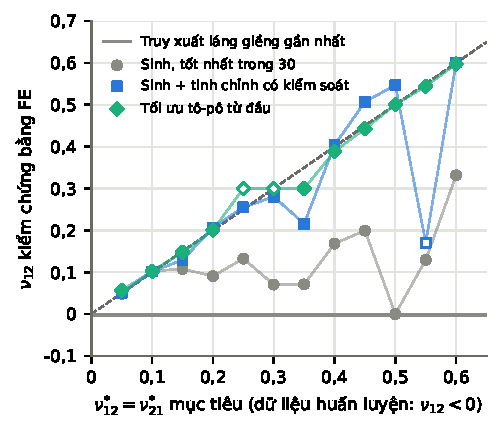
\includegraphics[width=0.5\linewidth]{figures/fig_signflip_vi.pdf}
\caption{Mục tiêu đổi dấu đối xứng: $\nuot$ kiểm chứng FE của pipeline sinh
(best-of-30 và sau tinh chỉnh có kiểm soát) và của tối ưu tô-pô chạy từ đầu.
Truy xuất bị chặn bởi thư viện huấn luyện ($\nuot\le-0,002$, đường xám).
Điểm rỗng: thiết kế suy biến. Nét đứt: đường đồng nhất.}
\label{fig:signflip}
\end{figure}

\paragraph{Theo biên độ: tinh chỉnh đi được vào vùng dữ liệu thưa nhưng không
xa hơn.}
Chúng tôi quét $\nuot^{*}\in\{-1,0;$ $-1,5;$ $-1,75;$ $-2,0;$ $-2,25;$
$-2,5\}$ ($\nuto^{*}=-0,05$) với mười lần rút mã ẩn độc lập mỗi mục tiêu và
chọn best-of-30 (Bảng~\ref{tab:ood}, Hình~\ref{fig:ood}). Dữ liệu huấn luyện
thưa dần từ trước khi tới giá trị nhỏ nhất: 88 mẫu có $\nuot<-1,5$, 14 mẫu có
$\nuot<-1,75$ và hai mẫu có $\nuot<-1,9$, tất cả là phép quay $90^{\circ}$
của các ô có $\nuto$ cực trị. Tinh chỉnh nhận biết nhị phân hóa đạt sai số
tương đối trung vị 0,3\% tại $-1,75$ và 1,2\% tại $-2,0$, đạt tiêu chí đặt
trước 8\% tại $-2,0$. Tuy vậy phân bố tại đây có hai cụm: sáu trong mười lần
lặp kết thúc dưới 1,7\%, bốn lần nằm trong khoảng 17--31\%. Từ $-2,25$ trở đi
mọi biến thể đều bão hòa, và tinh chỉnh không kiểm soát tệ hơn không tinh
chỉnh. Tinh chỉnh là tìm kiếm cục bộ trong không gian ẩn của bộ giải mã và
không thể tạo ra những biên độ mà bộ giải mã chưa từng học biểu diễn.

\begin{table}[t]
\centering
\caption{Quét biên độ dị hướng ($\nuto^{*}=-0,05$; best-of-30; 10 lần lặp mỗi
mục tiêu). Giá trị: trung vị sai số tương đối của $\nuot$ kiểm chứng FE. Dải
huấn luyện của $\nuot$ kết thúc tại $-1,95$.}
\label{tab:ood}
\small
\begin{tabular}{lcccccc}
\toprule
$\nuot^{*}$ & $-1,0$ & $-1,5$ & $-1,75$ & $-2,0$ & $-2,25$ & $-2,5$\\
\midrule
Best-of-30, không tinh chỉnh       & 0,5\% & 0,8\% & 3,6\% & 10,1\% & 15,6\% & 21,7\%\\
+ tinh chỉnh liên tục              & 1,3\% & 1,2\% & 3,5\% & 31,0\% & 41,6\% & 45,5\%\\
+ tinh chỉnh nhận biết nhị phân    & 0,4\% & 0,2\% & 0,3\% & \textbf{1,2\%} & 24,7\% & 28,8\%\\
+ nhận biết nhị phân, có kiểm soát & 0,1\% & 0,2\% & 0,3\% & \textbf{1,2\%} & 14,2\% & 20,0\%\\
\bottomrule
\end{tabular}
\end{table}

\begin{figure}[t]
\centering
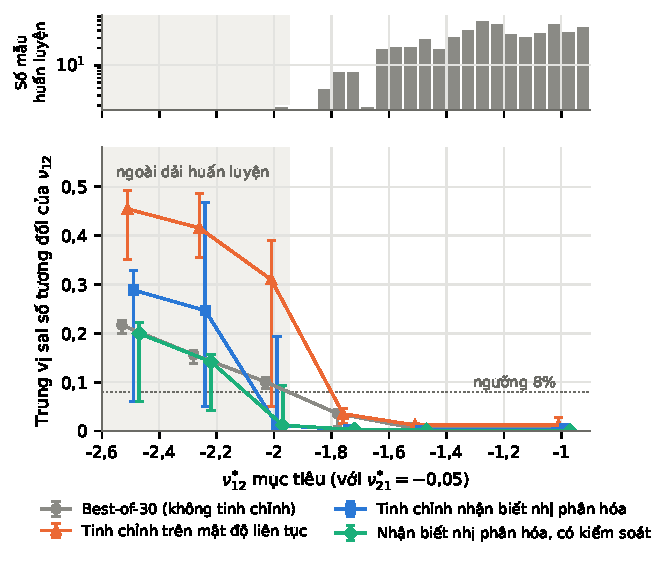
\includegraphics[width=0.62\linewidth]{figures/fig_ood_vi.pdf}
\caption{Trên: số mẫu huấn luyện theo khoảng $\nuot$ (thang log). Dưới: trung
vị sai số tương đối của $\nuot$ kiểm chứng FE theo mục tiêu
($\nuto^{*}=-0,05$). Thanh sai số: khoảng tứ phân vị trên 10 lần rút mã ẩn
mỗi mục tiêu; điểm được dịch ngang cho dễ đọc. Vùng tô: ngoài dải huấn luyện.
Chấm: tiêu chí đặt trước 8\% tại $\nuot^{*}=-2,0$.}
\label{fig:ood}
\end{figure}

\subsection{Thí nghiệm loại bỏ về kiến trúc}

\paragraph{Đầu KAN so với đầu tuyến tính.}
Chúng tôi thay ba lớp tuyến tính của cVAE (trung bình ẩn, log-phương sai và
nút cổ chai của bộ giải mã) bằng lớp Kolmogorov--Arnold \citep{liu2024kan}.
Hai loại đầu được huấn luyện với cùng công thức, siêu tham số và seed (123 và
7). KAN chỉ được coi là thắng nếu CI ghép cặp loại trừ 0 ở cả hai seed. Nó
không thắng ở chế độ nào (Bảng~\ref{tab:kan}). Ở chế độ production
(best-of-30 không tinh chỉnh), đầu tuyến tính tốt hơn có ý nghĩa ở cả hai
seed. Khi có tinh chỉnh, cả hai đều đạt $\RR(\nuot)=0,997$--$0,999$. Đầu KAN
có số tham số gấp $3,2$ lần (4,79\,M so với 1,49\,M) và cần khoảng $1,6$ lần
thời gian mỗi epoch, nên chúng tôi giữ đầu tuyến tính. Thí nghiệm này được
đánh giá với pipeline cũ có cân bằng cạnh tuần hoàn, vốn không làm thay đổi
độ chính xác trên tập A (Phụ lục~\ref{app:fp}).

\begin{table}[t]
\centering
\caption{Thí nghiệm loại bỏ có kiểm soát KAN so với tuyến tính trên tập A (hai
seed). $\Delta$MAE: mức giảm tương đối MAE($\nuot$) của KAN so với tuyến tính
(dương là có lợi cho KAN), CI 95\% bootstrap ghép cặp. In đậm: CI loại trừ 0.}
\label{tab:kan}
\small
\setlength{\tabcolsep}{4pt}
\begin{tabular}{lcccc}
\toprule
 & \multicolumn{2}{c}{$\RR(\nuot)$ Tuyến tính / KAN} & \multicolumn{2}{c}{$\Delta$MAE KAN so với tuyến tính}\\
\cmidrule(lr){2-3}\cmidrule(lr){4-5}
Chế độ & seed 123 & seed 7 & seed 123 & seed 7\\
\midrule
Mẫu đơn                 & 0,852 / 0,904 & 0,815 / 0,911 & $+13,3\%$ [$-0,2$; 24,4] & $\mathbf{+18,2\%}$ [3,8; 30,4]\\
Mẫu đơn + tinh chỉnh    & 0,994 / 0,997 & 0,998 / 0,999 & $+33,2\%$ [$-15,1$; 60,5] & $\mathbf{+33,9\%}$ [11,7; 52,3]\\
Best-of-30              & 0,977 / 0,974 & 0,982 / 0,980 & $\mathbf{-25,2\%}$ [$-56,2$; $-1,0$] & $\mathbf{-19,9\%}$ [$-42,1$; $-1,7$]\\
Best-of-30 + tinh chỉnh & 0,998 / 0,997 & 0,998 / 0,999 & $+11,3\%$ [$-38,7$; 43,6] & $\mathbf{+44,1\%}$ [24,9; 59,7]\\
\bottomrule
\end{tabular}
\end{table}

\paragraph{Bộ giải mã biểu diễn ẩn wavelet.}
Một bộ giải mã WIRE không phụ thuộc độ phân giải \citep{saragadam2023wire}
được thử một lần cuối. Nó kết hợp phép chiếu Heaviside trong hàm mất mát vật
lý, không ép đối xứng và công thức huấn luyện hai giai đoạn. Tiêu chí đặt
trước là tỉ lệ trúng mẫu đơn ít nhất 30\% và $\RR$ FE dương trên 24 mục tiêu
kiểm tra. Nó chỉ đạt tỉ lệ trúng 12,5\% và $\RR$ FE $-7,19$ sau best-of-30,
so với tỉ lệ trúng 100\% của bộ giải mã tích chập, và chỉ 4,6\% mẫu của nó
chế tạo được. Vì vậy chúng tôi đóng hướng này.

% ---------------------------------------------------------------------------
\section{Thảo luận}

\paragraph{Tối ưu chính cái được kiểm chứng.}
Phát hiện trung tâm là mọi phép tìm kiếm bằng gradient trên trường mật độ, dù
trong không gian ẩn của mô hình sinh hay trên mật độ phần tử của tối ưu
tô-pô, đều sẽ khai thác sự khác biệt giữa trường mà nó lấy đạo hàm và thiết
kế nhị phân cuối cùng được phân tích. Bộ tối ưu đạt hàm mục tiêu $10^{-10}$
trên những trường mà bộ kiểm chứng nhìn thấy rất khác (Hình~\ref{fig:gap}),
và điều tương tự xảy ra với tối ưu tô-pô dùng phép chiếu Heaviside tăng dần
tới $\beta=64$. Khoảng lệch này không thấy được trên đường cong mất mát. Từ
đó có ba cách khắc phục, đều rẻ: đưa các phép biến đổi kiểm chứng vào hàm
mục tiêu, chọn ứng viên theo sai số kiểm chứng thay vì sai số tối ưu, và coi
ô suy biến là thất bại ngay trong bộ kiểm chứng. Hai thành phần đầu không mới
trong tối ưu tô-pô theo mật độ \citep{guest2004achieving,wang2011projection};
điều bài báo này chỉ ra là bỏ qua chúng làm thay đổi kết luận của phép so
sánh giữa các phương pháp, và con đường sinh lẫn con đường kinh điển đều cần
chúng như nhau. Thành phần thứ ba dễ bị bỏ sót: một ô rỗng có hệ số Poisson
của vật liệu nền, và trong thí nghiệm đổi dấu, các ô như vậy là đáp án tốt
nhất mà tối ưu tô-pô trả về cho ba mục tiêu.

\paragraph{Mô hình sinh đóng góp gì.}
Khi so với tối ưu tô-pô hội tụ thay vì với bảng tra, lợi thế của pipeline
sinh hẹp hơn mức thường được ngầm hiểu, phù hợp với tổng quan phản biện của
\citet{woldseth2022use}. Nó đạt cùng độ chính xác kiểm chứng với số lần giải
FE mỗi mục tiêu ít hơn khoảng tám lần, và sai số cặp thấp hơn với mục tiêu dị
hướng vừa phải, nhưng khoản tiết kiệm chỉ được khấu hao sau hàng nghìn mục
tiêu vì chính dữ liệu huấn luyện được tạo ra bằng tối ưu tô-pô. Khi chưa tinh
chỉnh, truy xuất từ cùng thư viện cho độ chính xác tương đương. Vì vậy
pipeline hấp dẫn khi cần phục vụ nhiều mục tiêu, chẳng hạn trong thiết kế
tương tác hoặc vòng lặp trong của tối ưu đa thang, chứ không phải khi chỉ cần
một ô. Thất bại của nó có thể dự đoán được: mục tiêu dị hướng mạnh, vốn thưa
trong dữ liệu huấn luyện. Báo cáo thất bại theo tầng, thay vì gộp vào một
điểm số trung bình, đã giúp chúng hiện ra trong nghiên cứu này.

\paragraph{Khả năng chế tạo và mục tiêu ngoài phân phối.}
Tối ưu tô-pô chạy từ đầu tạo ô liên thông với kích thước nét đủ lớn thường
xuyên gấp hơn hai lần pipeline sinh. Tinh chỉnh không gian ẩn làm tăng nhẹ tỉ
lệ này, còn khởi tạo tối ưu tô-pô bằng thiết kế sinh ra không lấy lại được nó,
vì một phép chiếu khởi đầu sắc giữ nguyên tô-pô được sinh. Với mục tiêu không
auxetic, cVAE đạt đúng dấu ở nơi truy xuất từ thư viện không làm được, nhưng
tối ưu tô-pô đạt mục tiêu chính xác hơn nhiều. Theo biên độ, tinh chỉnh đẩy
được vào những vùng chỉ có vài mẫu huấn luyện, nhưng mọi biến thể sinh đều
dừng ở nơi dữ liệu kết thúc. Do đó các khẳng định ngoài phân phối cho mô hình
sinh nên nêu rõ hướng trong không gian tính chất, kiểm tra mục tiêu có khả
thi vật lý không, và so với tối ưu tô-pô thay vì với truy xuất. Ngoại suy biên
độ nhiều khả năng cần dữ liệu huấn luyện mới gần biên.

\paragraph{Giới hạn.}
(i) Độ chính xác được đo so với một mô hình FE $50\times50$ đàn hồi tuyến
tính, biến dạng nhỏ với $\nu_0=0,3$; sai số rời rạc hóa của nó (trung vị
0,015 về $\nuot$) lớn hơn các sai số trung bình được báo cáo. Biến dạng lớn,
vật liệu nền khác và ô ba chiều chưa được xét, và chưa thiết kế nào được thử
nghiệm thực tế.
(ii) Pipeline sinh thất bại với mục tiêu dị hướng mạnh ($r\ge10$), vốn thưa
trong dữ liệu huấn luyện; tối ưu tô-pô thì không.
(iii) Tối ưu tô-pô tạo ô chế tạo được thường xuyên gấp hơn hai lần (0,74--0,83
so với 0,32--0,35).
(iv) Với mục tiêu có dấu chưa thấy, tối ưu tô-pô chính xác hơn rõ rệt; lợi
thế của mô hình sinh trong vùng này chỉ đúng khi so với truy xuất.
(v) Lợi thế chi phí được khấu hao sau khoảng 3\,500 mục tiêu.
(vi) Điểm thẩm mỹ là một heuristic chưa được đối chiếu với đánh giá của con
người.
(vii) Phương pháp tinh chỉnh được chọn sau một thất bại trên tập A; việc tái
lập trên tập B và C cùng phép kiểm định đặt trước trên tập C làm giảm, nhưng
không xóa bỏ, sự phụ thuộc này.

\section{Kết luận}
Tinh chỉnh ô vật liệu meta được sinh ra bằng vật lý chính xác chỉ đáng tin cậy
khi hàm mục tiêu được tính trên chính thiết kế sẽ được kiểm chứng: đã nhị
phân hóa, đã lấy mẫu lại và đã kiểm tra suy biến. Với thay đổi này, một cVAE
kèm tinh chỉnh không gian ẩn ngang tối ưu tô-pô hội tụ về $\nuot$ với số lần
giải FE ít hơn khoảng tám lần và đạt sai số cặp thấp hơn với mục tiêu dị
hướng vừa phải, được tái lập trên ba tập mục tiêu rời nhau. Tối ưu tô-pô chạy
từ đầu vẫn là lựa chọn tốt hơn cho mục tiêu dị hướng mạnh, cho khả năng chế
tạo và cho mục tiêu ngoài dữ liệu huấn luyện. Cùng nguyên tắc đó áp dụng cho
chính tối ưu tô-pô: thứ cần được tối ưu và so sánh là thiết kế được kiểm
chứng, không phải trường mật độ đã chiếu.

\appendix
\section{Cân bằng cạnh tuần hoàn}
\label{app:fp}
Pipeline cũ thay các cột và hàng biên đối diện bằng trung bình của chúng
trước khi lấy ngưỡng, cả lúc kiểm chứng lẫn bên trong tinh chỉnh, và tính độ
lệch cạnh vào điểm chế tạo. Vì lưới FE dùng điều kiện biên tuần hoàn trên
phần tử, mọi ô điểm ảnh đều lát kín bằng phép tịnh tiến và bước này là không
cần thiết. Nó còn đẩy tính chất kiểm chứng của ô huấn luyện ra xa nhãn (MAE
$\nuot$ 0,055 khi có bước này, 0,032 khi không). Trên tập A, bỏ bước này
không làm thay đổi độ chính xác sau best-of-30 và tinh chỉnh. Quyết định bỏ
được đưa ra trước khi tính lại các số liệu của bài; sau đó nhiều kết quả tốt
lên, nên cả hai phiên bản đều được báo cáo. Thay đổi chính (có $\to$ không):
$\Delta$MAE tinh chỉnh mẫu đơn $+91,8\%\to+92,7\%$; $\Delta$MAE tinh chỉnh
sau best-of-30 $+62,6\%\to+68,3\%$; tỉ lệ chế tạo được sau best-of-30 và tinh
chỉnh có kiểm soát $0,24\to0,32$ (đã bỏ tiêu chí cạnh khỏi định nghĩa); quét
biên độ tại $\nuot^{*}=-2,0$, tinh chỉnh nhận biết nhị phân hóa,
$12,5\%\to1,2\%$; lợi thế sai số cặp khi $r<10$ trên tập C $+27\%\to+35\%$,
lợi thế $\nuot$ $+19\%$ (CI chứa 0) $\to+37\%$; Spearman trung bình của điểm
tổng hợp $0,693\to0,718$. Các kết quả có tiêu chí đặt trước (phép kiểm định
phân tầng trên tập C, phương án lai) là kết quả thu được khi còn bước này.

% ---------------------------------------------------------------------------
\section*{Tuyên bố}

\paragraph{Tái lập kết quả.}
Mã nguồn (sinh dữ liệu, đồng nhất hóa FE với độ nhạy chính xác, huấn luyện
cVAE, tinh chỉnh, baseline tối ưu tô-pô), các checkpoint đã huấn luyện, các
tập mục tiêu và mọi đầu ra theo từng mục tiêu làm cơ sở cho bảng và hình sẽ
được công bố tại [URL kho mã và DOI Zenodo - sẽ bổ sung]. Mọi con số trong bài
được sinh bởi các script trong \texttt{docs/paper1/scripts} từ các đầu ra này.

\paragraph{Tài trợ.} [Sẽ bổ sung.]

\paragraph{Xung đột lợi ích.} Tác giả tuyên bố không có xung đột lợi ích.
[Cần xác nhận.]

\paragraph{Sử dụng AI tạo sinh.} [Tác giả hoàn thiện: công cụ AI (Claude,
Anthropic) được dùng hỗ trợ phát triển mã, phân tích dữ liệu và soạn bản
thảo; tác giả đã rà soát toàn bộ nội dung và chịu hoàn toàn trách nhiệm.]

\paragraph{Đóng góp của tác giả.} [Sẽ bổ sung theo CRediT.]

\bibliographystyle{unsrtnat}
\bibliography{refs}

\end{document}
